\documentclass[conference]{IEEEtran}
\IEEEoverridecommandlockouts
% The preceding line is only needed to identify funding in the first footnote. If that is unneeded, please comment it out.
\usepackage{cite}
\usepackage{amsmath,amssymb,amsfonts}
\usepackage{multicol}
\usepackage{algorithmic}
\usepackage{graphicx}
\usepackage{textcomp}
\def\BibTeX{{\rm B\kern-.05em{\sc i\kern-.025em b}\kern-.08em
    T\kern-.1667em\lower.7ex\hbox{E}\kern-.125emX}}
\begin{document}

\title{Thread Pool in GeckoDB/BOLSTER - Integrating a Thread Pool into a high performance Database System \\
}

\author{
	\IEEEauthorblockN{Robert Jendersie}
	\IEEEauthorblockA{\textit{Otto-von-Guericke University} \\
		Magdeburg, Germany \\
		robert.jendersie@ovgu.de} \and

	\IEEEauthorblockN{Johannes Wuensche}
	\IEEEauthorblockA{\textit{Otto-von-Guericke University} \\
	Magdeburg, Germany \\
	johannes.wuensche@st.ovgu.de} \and

	\IEEEauthorblockN{Johann Wagner}
	\IEEEauthorblockA{\textit{Otto-von-Guericke University} \\
	Magdeburg, Germany \\
	johann.wagner@st.ovgu.de} \and

	\IEEEauthorblockN{Marten Wallewein-Eising}
	\IEEEauthorblockA{\textit{Otto-von-Guericke University} \\
	Magdeburg, Germany \\
	marten.wallewein-eising@st.ovgu.de}
}


\maketitle

\begin{abstract}

\end{abstract}

\begin{IEEEkeywords}
Thread Pool, GeckoDB, BOLSTER
\end{IEEEkeywords}

\section{Introduction}
Since the amount of data that is stored and processed by modern database systems is growing fast, sequential data processing as only possibility is inconceivable. Applications have to process data in parallel to reach sufficient throughput to fulfil appropriate requirements. 

Parallel data processing can be achieved by different approaches like instruction and data parallelism or multi threading. In this paper, we focus on multi threading by implementing a thread pool for the graph database system GeckoDB. The thread pool will be integrated into BOLSTER, a high performance library for parallel execution of primitives like for or filter on large data sets. In the current implementation, BOLSTER creates a fix number of threads for each call of a primitive. This approach is called \emph{thread-per-request}. Since many primitives are executed at the same time, many drawbacks arise from this implementation. 
First of all, the creation of threads comes along with overhead like stack initialisation and memory allocation. Secondly, creating a huge number of threads simultaneously may lead to large context switch overhead of the scheduler. Additionally, debugging and profiling applications that create many threads during runtime is 	time-consuming.

To overcome these drawbacks, we integrate an optimised thread pool in BOLSTER. Along with the implementation, we measure the performance of the primitives to determine the thread pool overhead. Additionally, we measure metrics like \emph{idle and job time} of threads to evaluate correct thread pool sizes for the considered use cases.  In this work we make the following contributions:
\begin{itemize}
	\item We describe our design and implementation of the thread pool 
	\item We evaluate the possibility to wait for a group of task in the calling thread
	\item We compare our thread pool against the existing implementation in BOLSTER
\end{itemize}
We organized the rest of the paper as follows. In Section 2, we give preliminaries about the considered task configuration and about thread safe access of memory. In Section 3, we show our design and implementation of the thread pool and examine our experimental environment in Section 4. In Section 5, we describe the results of our performance evaluation. In Section 6, we name related work and state our conclusion and future work in Section 7.

\section{Preliminaries}
In this section, we define our configuration of tasks that are processed by the thread pool and state difficulties of synchronizing thread access to memory.

\begin{figure*}[htbp]
	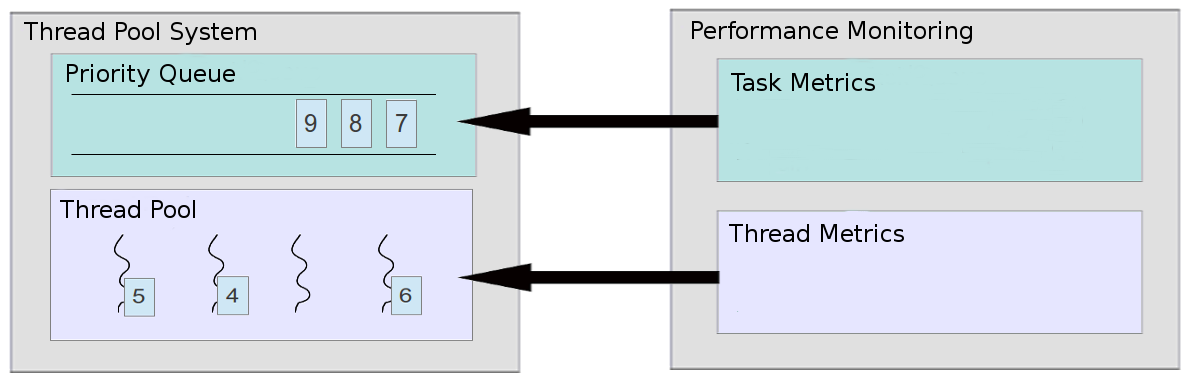
\includegraphics[width=1.0\textwidth]{img/pool_structure.png}
	\caption{Design of the thread pool system}
	\label{fig0}
\end{figure*}

\subsection{Task Configuration}
We define a Task as a structure containing data that has to be processed and an operation that has to be executed on the data. In this work, we define tasks as \emph{independent}, which means tasks do not have dependencies on other tasks and can be processed independently. Furthermore, we expect the data passed to two tasks are stored in different memory locations. Consequently, while executing the task operation, threads do not access the same memory locations. 

Each task can be enqueued with a priority. The priority zero is the highest and the task will be processed by the next free thread. The higher the priority of the task is, the further it is placed behind in the queue. Additionally, we only consider not preemtable tasks. Once a task is assigned to a thread, the thread will finish the operation of the task before getting a new one. 

\subsection{Synchronizing Memory Access from Threads}
Parallelism with multi threading works great as long as each thread works on a separate memory area. During task scheduling, the scheduler has to know the state each thread has. This can be solved with signal handling or by writing the current thread state into main memory. In this work, we implement the second approach to avoid having another thread that only schedules tasks to other threads. 

Threadsafe access to memory can be achieved by different approaches. Firstly, a mutex thread can manage the access for multiple other threads. Secondly, atomic operations ensure the safe access from different threads to the same memory. We use both approaches for different parts of the thread pool. Since using a mutex thread can decrease access performance, we decided to execute atomic operations on the memory containing the thread state informations. For example, the function \emph{atomic\_compare\_exchange\_strong} performs a compare and, if the result is true, an exchange of the memory in one atomic operation. We use a mutex thread to synchronize the enqueueing of tasks into the priority queue.

%\begin{figure}
%	\includegraphics[width=0.4\textwidth]{figure_1.png}
%	\caption{Coherence between data, instructions, and the results of SISD and SIMD.}
%	\label{fig}
%\end{figure}
% SIMD explanation

%\begin{table*}[htbp]
%	\caption{SIMD instructions from Streaming SIMD Extensions 2 (SSE2)}
%	\begin{center}
%		\begin{tabular}{|c|c|}
%			\hline
%			\textbf{SIMD instruction}&\textbf{Explanation}\\
%			\hline
%			\_\_m128i \_mm\_load\_si128 (\_\_m128i *p) & Loads a 128-bit value. Returns the value loaded into a variable representing a register.\\
%			\_\_m128i \_mm\_cmpgt\_epi32 (\_\_m128i a, \_\_m128i b) & Compares 4 signed 32-bit integers in a and 4 signed 32-bit integers
%			in b for greater-than.\\
%			\_\_m128i \_mm\_set1\_epi32(int i) & Sets the four signed 32-bit integer values to i.\\
%			\hline
%		\end{tabular}
%		\label{tab1}
%	\end{center}
%
%\end{table*}

\section{Implementation}
In this section, we describe in detail the design and implementation of our thread pool. We show how tasks are enqueued regarding their priority and how the scheduling is implemented. Additionally, we state our thread metrics and how they are integrated in the thread pool design. 

\subsection{Architecture of the Thread Pool}
Compared to simply create threads on demand, managing threads in a pool comes along with memory and CPU overhead. The thread pool must know information about the state each thread has and his assigned task. To measure metrics of threads and tasks, additional memory for threads and tasks is required. 

In Figure 1, we show our design of the whole thread pool system, containing the thread pool itself, the task priority queue and the performance monitoring. Since measuring performance metrics lead to memory and CPU overhead, we decided to exclude the performance measurements from the thread pool to make it optional. The performance monitoring can be activated with an additional function call of \textbf{TODO: Insert function here}. Consequently, in the target database system, the designers can decide for each thread pool instance, if performance monitoring should be applied. 

The thread pool system includes an array of threads and a priority queue to store the passed tasks. We decided to implement the thread pool using the POSIX thread library to provide the thread pool for multiple operation systems like Linux and Unix. Additionally, we avoid using custom compiler flags to ensure that the thread pool can be compiled with different compilers. The thread pool itself contains a variable number of threads. Since XY and XZ show the importance of accurate thread pool size, we add a resizing function for our thread pool, which enables to change the amount of threads at runtime. 

\subsection{Thread Pool and Task Queue}
Threads and tasks are two major entities in the thread pool system. As we can observe from Figure 1, thread pool and task queue are two data structures used to store the required information related to the threads and the submitted tasks, respectively. Each spawned thread can be either working on a task or waiting for the next task. Consequently, we define the states of a thread to \emph{busy} and \emph{waiting}. 

\subsection{Enqueueing Tasks}
\begin{figure}
	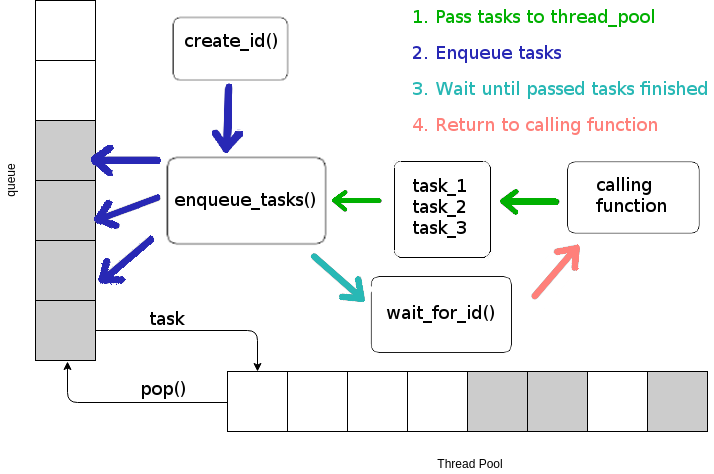
\includegraphics[width=0.5\textwidth]{img/pool_queue.png}
	\caption{Workflow of task enqueueing and execution in the thread pool}
	\label{fig1}
\end{figure}

\subsection{Waiting for Tasks}
\begin{figure}
	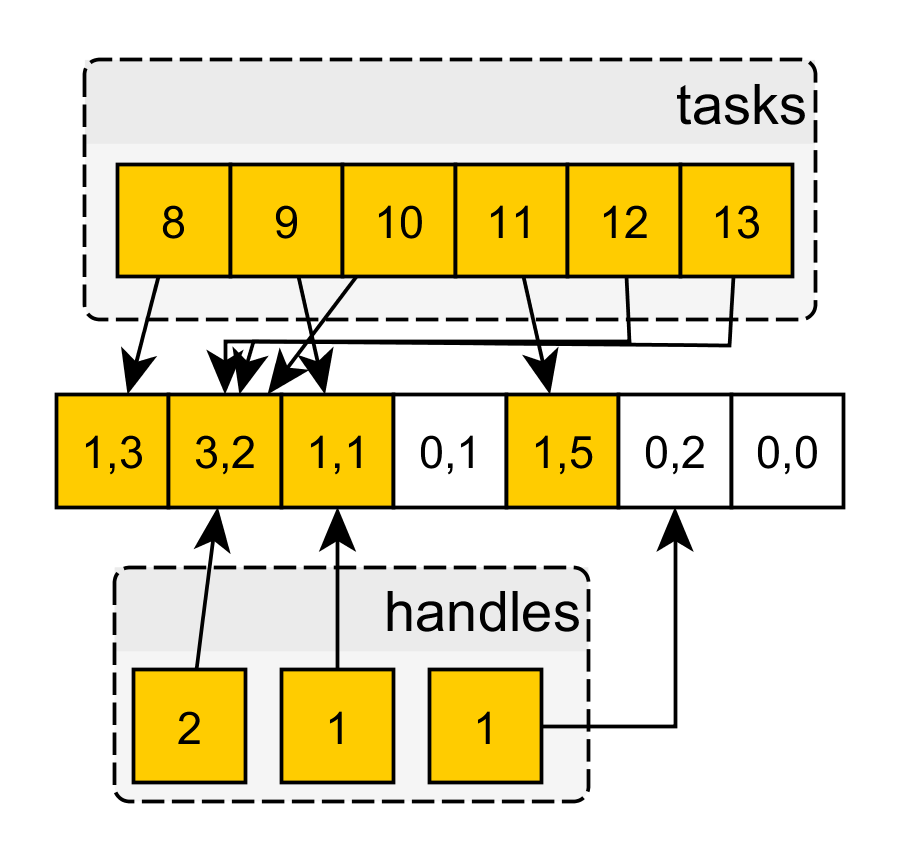
\includegraphics[width=0.5\textwidth]{img/waitingconcept.png}
	\caption{Concept of waiting for tasks using a slotmap}
	\label{fig2}
\end{figure}
As mentioned in the previous section, ids are assigned to the tasks before they are enqueued. 

\subsection{Managing Thread States}
- To handle the shrinkage of the pool while threads are processing tasks, we change the state

\subsection{Thread metrics}

\section{Experimental Environment}

\section{Evaluation}

\section{Related Work}

\section{Conclusion and Future Work}
\cite{pyarali2001evaluating}
\bibliographystyle{splncs}
\bibliography{paper_thread_pool} 

\end{document}
